\documentclass{article}

\usepackage{amsmath,amssymb}
\usepackage{geometry}
\usepackage{graphicx}

\geometry{a4paper, margin=2.5cm}

\begin{document}

% ============================================================
\section*{The Decision Transformer (DT)}

\subsection*{First, a story}

Chapter 9's ending left a fork in the road: facing offline data that can no longer be queried, CQL and IQL chose to write pessimism into the value function, safely extrapolating estimates beyond the data. But around 2020, another field was having a revolution: GPT proved that, given enough data, the purely supervised objective of ``next-token prediction'' learns strikingly complex behavior. So someone asked a cross-disciplinary question: \textbf{if sequence modeling is this strong, why do we still need the Bellman equation?}

\textbf{The naive approach}: treat trajectories as sentences and actions as tokens, training $P(a_t \mid s_t, \text{history})$ --- which is behavior cloning (BC), Chapter 9's pass line: the policy matches the data's level, and control over output quality is lost.

\textbf{This chapter's way}: write the \textbf{desired return} into the sequence too. The trajectory is no longer a stream of $(s, a)$ but of $(\hat R, s, a)$ --- the model learns ``given that I want return $\hat R$, what action should I take''. At evaluation, set $\hat R$ to the target score and order a return level like requesting a song.

\textbf{The core question}: is this \textbf{planning}, or \textbf{retrieval} of trajectories seen in training?

\[
\boxed{P(\tau) = \prod_{t} P\!\left(a_t \,\Big|\, \hat{R}_{t-K+1:t},\; s_{t-K+1:t},\; a_{t-K:t-1}\right)}
\]

\subsection*{Formalization}

A trajectory is serialized into an alternating return--state--action stream:

\[
\tau = \left(\hat{R}_1, s_1, a_1,\; \hat{R}_2, s_2, a_2,\; \ldots,\; \hat{R}_T, s_T, a_T\right)
\]

where $\hat{R}_t$ is the \textbf{return-to-go (RTG)}: the reward sum from step $t$ to the end,

\[
\hat{R}_t = \sum_{k=t}^{T} r_k
\]

(the discounted version $\sum_{k\ge t}\gamma^{k-t}r_k$ is analogous; this chapter's experiments use $\gamma=1$.) The DT is a causal Transformer: the $t$-th token encodes $(\hat{R}_t, s_t, a_{t-1})$, attends only to the past, and outputs a distribution over $a_t$. Training is pure supervised cross-entropy --- no Bellman equation, no bootstrapping, no $\max$, no value function:

\[
\mathcal{L}(\theta) = -\,\mathbb{E}_{\tau \sim \mathcal{D}}\left[\sum_t \log P_\theta\!\left(a_t \,\Big|\, \hat{R}_{t-K+1:t}, s_{t-K+1:t}, a_{t-K:t-1}\right)\right]
\]

with $K$ the context length (16 here). The evaluation protocol is the chapter's ``remote control'': feed the target $\hat{R}_1 = \text{target}$ at the first step, then recurse by definition,

\[
\hat{R}_{t+1} = \hat{R}_t - r_t
\]

The model outputs actions, the environment returns rewards, and RTG decreases accordingly --- not a single value estimate anywhere in the loop.

% ============================================================
\section*{Core mechanisms}

\subsection*{Mechanism 1: RTG conditioning --- return as command, valid only within the data}

RTG turns ``policy quality'' into an input: one model, $\hat R$ of 50 is a passing policy, 450 an excellent one. Figure~1 (left) verifies this on mixed-quality data (the full spectrum from random to expert): for targets $\ge 200$ the evaluated return tracks the target closely (200 $\to$ 210, 300 $\to$ 286, 500 $\to$ 335); in the low range (50--100) it only reaches 10--33 --- doubly bounded by CartPole's achievable floor (a random policy is $\approx 9$) and the data density of low-return behavior. As a control, the same architecture trained without RTG input (i.e., sequence BC) pins at about 10 (measured 9.5, the random level) no matter how much return is requested --- \textbf{without RTG, the return cannot be specified}.

But the baton's range is drawn by the data. Figure~1 (right) pushes targets beyond the data's best: 600--1000 brings no further gain (returns 259--339 with exploding variance) --- the target itself becomes an input dimension that can go out of distribution, the same notion as the reward model's ``coverage zone'' in Chapters 12 and 13: \textbf{conditional generation works only near conditions it has seen}.

\begin{figure}[!htbp]
  \centering
  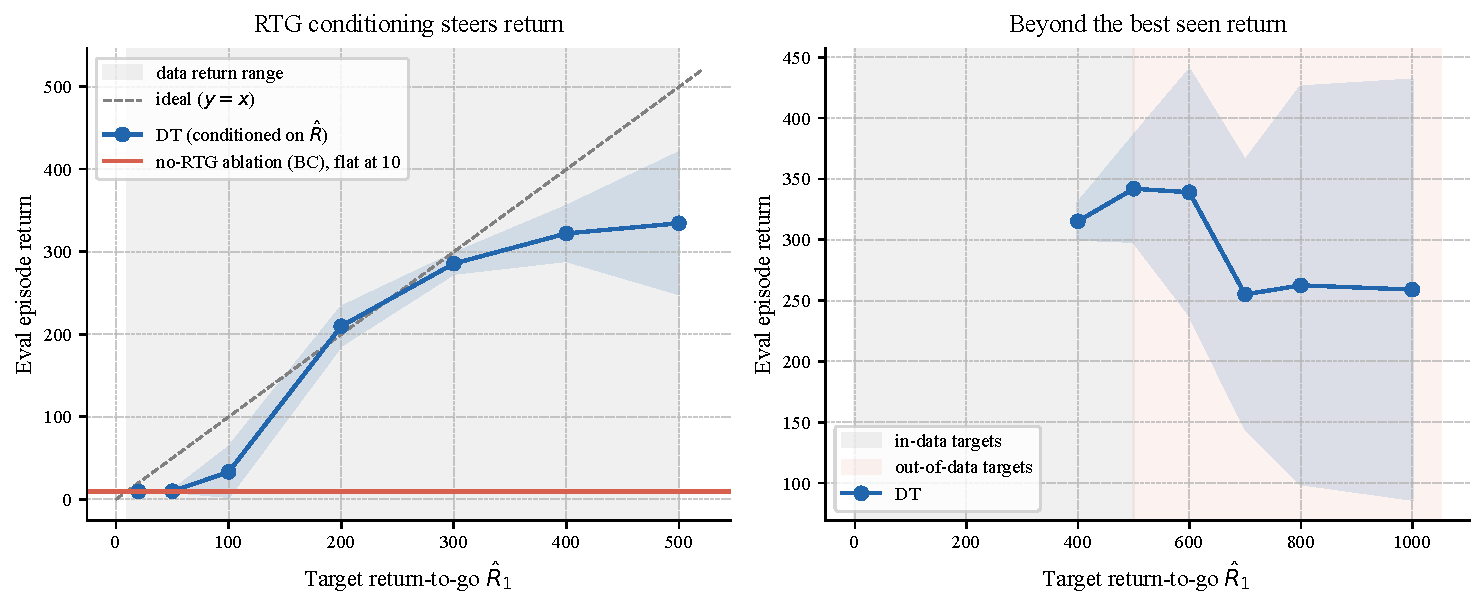
\includegraphics[width=0.98\textwidth]{fig1_rtg_conditioning.pdf}
  \caption{RTG conditioning (CartPole-v1 mixed-quality data, 3 random seeds, mean $\pm$ std). Left: DT (blue) tracks the target (dashed $y=x$; gray is the data return range); the no-RTG model of the same architecture (red) pins at a fixed level --- the return cannot be specified. Right: beyond the data's best return the DT cannot deliver and even falls back --- conditioning is valid only within the data's support.}
  \label{fig:dt-rtg}
\end{figure}

\subsection*{Mechanism 2: the data-quality ceiling --- replay, not improvement}

Train DT and BC separately on three data tiers (random / medium / expert, collected with Chapter 9's recipe). Figure~2's bars give a crisp conclusion: random tier, data mean 22, DT 44, BC 10; medium, 211 / 267 / 262; expert, 361 / 352 / 347 (one seed's collection policy stalled at 102, dragging down the data mean and widening the error bars --- model quality follows data quality seed by seed) --- \textbf{sequence modeling replays data; it does not improve it}. The DT--BC difference is not capability but controllability: DT holds a baton, yet the ceiling is the data itself.

Together with Chapter 9: CQL and IQL extrapolate values beyond the data via pessimism and recover above BC on medium data; DT simply does not extrapolate. This yields a clear selection rule: when the \textbf{data is near-optimal} (demonstrations, expert trajectories), DT is simple, stable, and controllable --- exactly SFT's situation in LLM post-training; when the \textbf{data is suboptimal and must be exceeded}, value methods are irreplaceable.

\begin{figure}[!htbp]
  \centering
  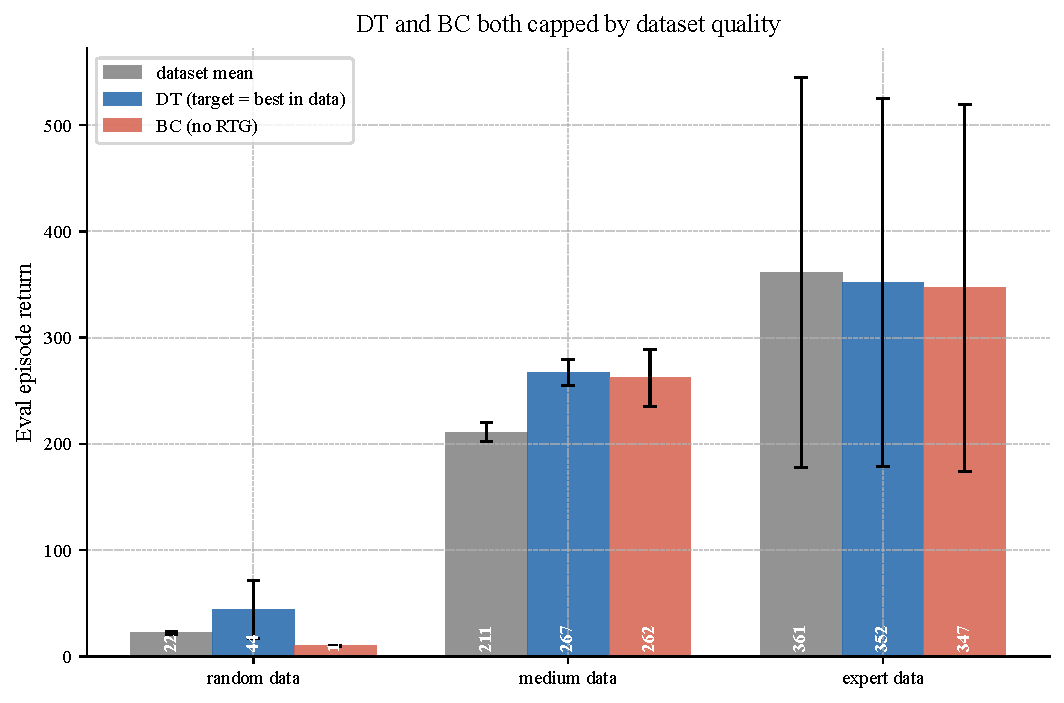
\includegraphics[width=0.88\textwidth]{fig2_data_quality.pdf}
  \caption{The data-quality ceiling (CartPole-v1, three data tiers $\times$ 3 random seeds, error bars $\pm 1\sigma$). DT (evaluation target set to the data's best return) and BC both hug the data's average level; neither exceeds the data quality --- contrast CQL/IQL in Chapter 9 recovering above BC on medium data.}
  \label{fig:dt-quality}
\end{figure}

\subsection*{Mechanism 3: stitching failure --- retrieving the seen, not composing the unseen}

``Stitching'' is offline RL's distinctive demand: every transition of the optimal trajectory is in the data, just \textbf{never within a single trajectory} --- joining the first half of trajectory A with the second half of B at a shared state yields behavior better than anything in the data. Chapter 2's dynamic programming stitches naturally: value iteration's wave propagates across trajectories, and backups never ask where a transition came from. Sequence modeling does not: its context is ``history within one trajectory''; pattern matching retrieves whole sequences it has seen.

The experiment lays this bare (Figure~3): a deterministic $8\times 8$ grid world, shortest path 14 steps; 400 data trajectories whose best is 16 steps --- the 14-step path never appears whole, yet every transition it needs is in the data. The result: tabular \textbf{offline Q-learning stitches the 14-step optimum from the same data} (all three seeds); the DT delivers normally for targets $\ge 22$, degrades entering the data-sparse region at $\le 20$, and conditioning on the never-seen 14 fails in 60 of 90 evaluation episodes.

\begin{figure}[!htbp]
  \centering
  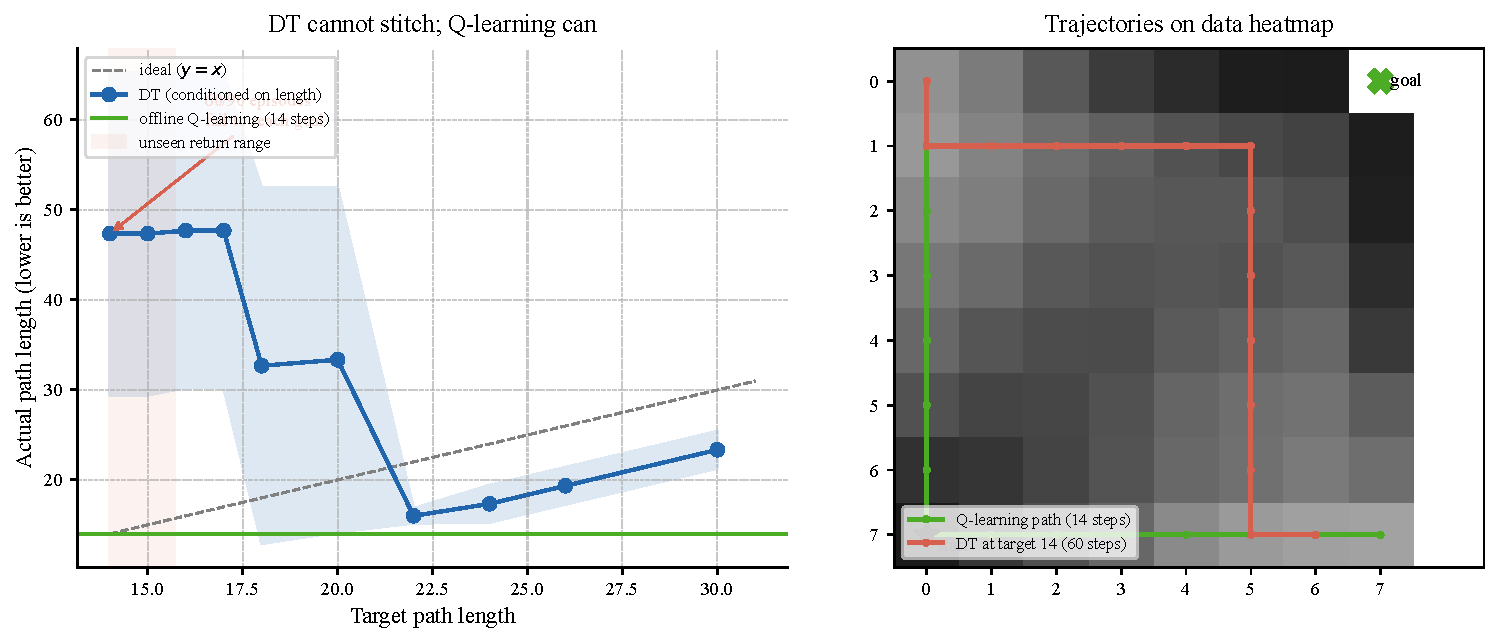
\includegraphics[width=0.98\textwidth]{fig3_stitching.pdf}
  \caption{Stitching failure (deterministic $8\times 8$ grid world, 3 random seeds, mean $\pm$ std). Left: for target lengths $\ge 16$ (the data's best) the DT (blue) delivers; conditioning on the optimal 14 steps (red region --- the return falls outside the data's support) the DT fails, while offline Q-learning (green) stitches the 14-step optimum from the same data. Right: the data visit heatmap and path comparison --- Q-learning's diagonal shortcut is stitched across trajectories; the DT's actual trajectory at target 14 misses the optimum.}
  \label{fig:dt-stitch}
\end{figure}

% ============================================================
\section*{The full algorithm}

\begin{enumerate}
  \item \textbf{Serialize}: write each trajectory as a $(\hat R_t, s_t, a_t)$ stream; standardize states by the data's mean/variance and scale RTG by the data's maximum return;
  \item \textbf{Train}: sample windows of length $\le K$ (right-aligned) and minimize the action cross-entropy --- pure supervision, no environment interaction;
  \item \textbf{Evaluate}: initialize $\hat R_1 = \text{target}$; each step take the action greedily (or by sampling) and recurse $\hat R_{t+1} = \hat R_t - r_t$; keep the last $K$ tokens as context.
\end{enumerate}

Practical notes: keep the target return \textbf{within the data's range} (this sits beside RLHF's $\beta$ and DPO's training steps as a ``hidden hyperparameter'' --- set it too high and you get Figure~1's OOD failure); the context length $K$ trades long-horizon credit against training cost; with $K=1$ the DT degenerates to the simplest conditional imitation.

% ============================================================
\section*{Comparison with neighbors}

\begin{center}
\begin{tabular}{c|c|c|c}
 & \textbf{BC} & \textbf{CQL / IQL} & \textbf{DT} \\
\hline
Learning signal & supervised imitation & Bellman + pessimism & supervised + RTG conditioning \\
Can exceed the data & no & yes (extrapolated values) & no (replays the data) \\
Can stitch & no & yes (cross-trajectory backups) & no (within-trajectory retrieval) \\
Controllability (specify return) & none & none & yes (within the data range) \\
Key hyperparameters & none & $\alpha$ / $\tau$, $\lambda$ & target RTG, context $K$ \\
Best suited for & data is the goal & suboptimal data to be exceeded & near-optimal data + controllability \\
\end{tabular}
\end{center}

\textbf{In one sentence}: value methods answer ``what is it worth beyond the data''; sequence methods answer ``what does it look like within the data'' --- the two philosophies of offline RL, each irreplaceable.

% ============================================================
\section*{Where this chapter sits in the RL landscape}

\begin{enumerate}
  \item \textbf{Upstream}: offline RL (Chapter 9) supplies the problem and the pathology --- distribution shift, extrapolation error, the BC pass line; this chapter answers the same question with a different worldview (sequence modeling);
  \item \underline{The Decision Transformer} (this chapter: RL as sequence modeling --- return is the condition, action is the generation; three mirrors delimit it: conditions can go OOD, data is the ceiling, no stitching);
  \item \textbf{Downstream}: the language models of Chapters 12--14 (RLHF, DPO, GRPO) are the same species as this chapter's DT --- ``sequence modeling + conditional generation'' is the carrier of every post-training method; the differences are only in what the condition is (preferences, log-ratios, verifiable rewards) and where the objective comes from.
\end{enumerate}

The takeaway: \textbf{DT proves that sequence modeling suffices to reproduce the intelligence in the data --- and precisely only that far; exceeding the data still requires values and planning}. From the next chapter on, this ``species'' of sequence model faces its most important conditional input: human preferences.

\subsection*{References}

\begin{enumerate}
  \item Chen et al.\ (2021). Decision Transformer: Reinforcement Learning via Sequence Modeling. \textit{NeurIPS}.
  \item Janner et al.\ (2021). Offline Reinforcement Learning as One Big Sequence Modeling Problem. \textit{NeurIPS}.
  \item Brandfonbrener, Whitney \& Kakade (2022). When Does Return-Conditioned Supervised Learning Work for Offline Reinforcement Learning? \textit{NeurIPS}.
  \item Emmons et al.\ (2022). Where Did the Distribution Shift? A Causal Analysis of Behavior Cloning and Offline RL. \textit{NeurIPS}.
  \item Levine et al.\ (2020). Offline Reinforcement Learning: Tutorial, Review, and Perspectives on Practical Applications. \textit{arXiv:2005.01643}.
\end{enumerate}

\end{document}
